\documentclass[10pt]{article}

\title{Project 3}
\author{Noah Salomons, 114132239}
\usepackage[margin=0.7in]{geometry}
\usepackage{graphicx}
\usepackage{amsmath}

\begin{document}
\maketitle

\section{Part 1 - Setting Up Local Classifiers}
\subsection{Local Windows}
First, the user creates a rough outline of the foreground image they want to track in the first image. I turned this into an outline and used the $improfile$ function to get equidistant windows along this outline. The size of each window is 51x51 - chosen by experimentation and by taking some suggestion from the paper "Video SnapCut: Robust Video Object Cutout Using Localized Classifiers" by Bai, Wang, Simons, and Sapiro (referenced later as "SnapCut Paper"). The amount of windows changes from input to input. The amount is the number of pixels in the outline divided by 20. This ensured sufficient overlap between windows. Overlap is necessary to make sure that there is no gaps when recreating the foreground mask for subsequent images. Windows were stored by keeping track of each window's top left corner, bottom right corner, and its center. The center was found first using $improfile$ and then the corners were found by adding/subtracting 25. If anything was out of bounds, the center was adjusted.
\subsection{Initializing the Color Model}
Next I created the initial color models. These are used to map and compare the color of the foreground relative to the background. Combined with the other models created later, they let us see where the foreground is and isn't based on color. The following process was repeated for every window. First, I found the local foreground mask, or the foreground that is visible in the current window. When using this mask and its inverse for the background, I made sure not to use pixels that were close to the boundary to ensure I was sampling pixels in the foreground or background, respectively. I converted the first image to Lab color space. Using the $fitgmdist$ function, I trained two GMMs for the current window: one for the foreground and one for the background. The input was a $m$ by 3 matrix where each column corresponded to the values in the L, a, or b color space in the foreground (or background). Then, I used the $pdf$ function to create probability density functions for the foreground and background GMMs of that window. The color model was formed by dividing each pixel's value in the foreground pdf by the sum of its values in the foreground and background pdfs. Again, this was repeated for every window and stored. I also stored the pdfs used because they were needed later.
\subsection{Color Confidences}
For each window's color model, there is a color confidence. These are used in deciding how much to "trust" the color model when determining the location of the foreground about the future images. Getting these color confidences was relatively easy. For every window I solved the following equation (Equation 2 in the SnapCut Paper): $f_c = 1 - \frac{\sum_{all pixels} |L^t(x) - p_c(x)|\cdot w_c(x)}{\sum_{all pixels} w_c(x)}$. In the equation, $f_c$ is color confidence, $L^t(x)$ is the value of pixel $x$ in the foreground mask (0 or 1), $p_c(x)$ is the value of pixel $x$ in the color model, $w_c(x) = e^{\frac{-d^2(x)}{\sigma_c^2}}$, $d(x)$ is the distance from pixel $x$ to the foreground boundary according to the distance transform, and $\sigma_c$ is half the window distance.
\subsection{Shape Model and Shape Confidence}
Next I created the shape models, which is created using shape confidence. As the color confidence decreases, shape confidence increases. Basically the less we trust the color model, the more we should trust the shape model. Again, creating the shape models were as easy as solving equations provided in the SnapCut Paper. For every window we do the same thing. The value of a pixel in the corresponding shape model of a window is calculated as $1 - e^{\frac{-d^2(x)}{\sigma_s^2}}$. If the color confidence for the window is $\leq 0.85$, then $\sigma_s = 2$ (as specified in the SnapCut Paper). Otherwise, $\sigma_s = 2 + (\frac{windowsize - 2}{1 - 0.85})^2(f_c - 0.85)^2$ where $f_c$ is the color confidence of the window. As shown later, the shape model and color model are used to estimate the location of the foreground in future frames after estimating motion.
\\\\
NOTE: Everything from this point forward was repeated for all images (except the first one).
\section{Part 2 - Updating Window Locations}
Now that we have our initial classifiers, we can move on to the next image. There were two steps to updating the window locations. Estimating rigid motion and optical flow.
\subsection{Estimating Whole-Object Motion (Rigid Motion)}
Estimating the motion of the whole object was as simply as detecting features (using $detectHarrisFeatures$), extracting features, matching the features, and estimating the affine transform (using $estimateGeometricTransform$). $detectHarrisFeatures$ worked well for some image sets, but not for others. I eneded up switching to $detectSURFFeatures$ with a metric threshold of 100. This gave better results for all image sets. Then, for each window, I transformed each center point by the previously calculated affine transform. Finally, I recalculated the top left and bottom right points based on the center point to reform the 51 by 51 window. One issue I had was that the affine transformation was inaccurate. After visualizing the matches that were being made, I noticed that in some image sets the background was matching a lot. Using the "ROI" parameter in $detectSURFFeatures$ to only detect features within a box around the foreground fixed this problem and resulted in a better output.
\subsection{Estimating Local Boundary Deformation (Optical Flow)}
The previous step only accounted for the movement of the foreground object as a whole. However, often individual parts of an object can move different from the whole. We can use optical flow to estimate these individual movements. Using an $opticalFlowFarneback$ object, I used the $estimateFlow$ function to estimate the optical flow of each pixel in the object. Then for each window, I calculated the average flow of all the pixels in the window to get one average $x$ and one average $y$ value for each window. These average $x$ and $y$ values were added to the center of each window and, again, the top left and bottom right corners were adjusted (while accounting for potential out of bounds scenarios).

\section{Part 3 - Updating Local Classifiers}
Now that we've updated the window locations, we can update the color and shape models for the current image.
\subsection{Updating the Color Model and Color Confidence Value}
The following process was repeated for every window. First, I retrieved the 51 by 51 section of the image in the Lab color space that corresponded to the current window. I used $fitgmdist$ again to train new GMMs for the foreground and background, but the input was different. I still used a $m$ by 3 matrix, but each column in the matrix used for the foreground GMM corresponded to the value of pixel in the L, a, and b color spaces that had a shape confidence value of $> .75$ in the corresponding shape model for that window. In the background GMM, the threshold was .25 rather than .75. I created new pdfs using these new GMMs. Next, I took the GMMs used in the previous frame to create new pdfs by using pixels in the current image. I combined these pdfs created with old GMMs with the ones that were created from the new GMMs by averaging them. I created a new color model for this window by dividing this new average foreground pdf by the sum of the average foreground and background pdfs and reshaped it. Then, I compared the number of pixels that are greater than 0 in this new color model to the one used in the previous frame. If the number of pixels that had a value of greater than 0 was more in the new color model, then the previous color model was used for the current frame. This is because if there is more pixels that are more than 0, the estimated foreground in the new color model is larger which means there is more potential for error. It's safer to just use the older one. However, if the number of pixels that had a value of $>$ 0 was less than in the old color model, we can update the color model. The color model for the current window was updated to be the new one. Additionally, since we changed the color model, we need to calculate a new color confidence value. This was done using the same method as before. Finally, the average foreground and background pdfs were stored because they will be used later.
\subsection{Updating the Shape Model and Shape Confidence Model}
The SnapCut Paper is not clear when they update the shape model and shape confidence model. However, it is clear that they do need to be updated. I chose to update them after updating the color model for a few reasons. First, updating the color model relies on the shape model from the previous frame, so they could not be updated before that. Addtionally, they needed to be updated before combining shape and color models. Therefore, the only logical place to update them was after updating color models and before combining them. Firstly, I used the affine transform from when rigid motion was estimated to warp the shape model into a new position that better resembles the current image and created a new distance transform. Next, I just created new shape confidence models for the current image using the same method as before. Note that if any of the window's color models were updated, the new shape confidence model for that window would use the updated color confidence, too.

\section{Part 4 - Combining Shape and Color Models}
Now that the color and shape models as well as the foreground mask have been updated, we can integrate them all together. For each window, the combined model was $f_s \cdot L^{t+1} + (1 - f_s) \cdot p_c$. The first part of the equation is the shape model for the current window multiplied by the foreground mask of the current window. The second is the opposite of the shape model multiplied by the color model for the window. Basically what this does is weight the foreground mask and color model based on the shape model. All the integrated models are white where the foreground is and fade off and are rough around the foregound/background edge where the color model is, but the foreground map isn't.

\section{Part 5 - Merging Windows and Extracting Final Foreground Mask}
\subsection{Merging Windows}
The first step I took in merging the windows was resizing each window to be the size of the whole image. In other words I just expanded the boundaries of the window so it was 0 everywhere except where the window wasn't and where the window didn't cover. This just allowed for easier merging. The following formula was used for merging $p_f(x) = \frac{\sum_k p^k_F(x) (|x - c_k| + \epsilon)^{-1}}{\sum_k(|x - c_k| + \epsilon)^{-1}}$. $\epsilon = 0.1$ because that's what was used in the SnapCut Paper. $x - c_k$, or distance of the pixel to the center of the window, was caluclated using Euclidean distance. I looped through every pixel. At each pixel, I looped through all the windows and if the original window covered that pixel, I added the respective value to the current numerator and denominator of that pixel. After iterating through every window, I divided the total numerator by the denominator to get the value for that pixel.
\subsection{Extracting Final Foreground Mask}
Merging all the windows still gave somewhat of a rough result. Most obviously, there's a hole in the middle of the mask where no windows covered. I used $imfill$ to fill the middle. $imfill$ also messed with the edges a bit, but it didn't have too much of an effect on the next step. I used $lazysnapping$ to get a tighter boundary around the foreground. I used $superpixels$ with 1000 segements (found by experimentation) for the second parameter and the filled in foreground mask and its negation for the third and fourth parameters. The resulting mask was what I used to create a boundary around the foreground. This mask sometimes missed small parts of the foreground and/or included parts of the background, but overall it worked pretty well.

\section{Part 6 - Conclusions}
\subsection{Overview of the Process}
Locations of local windows: \\
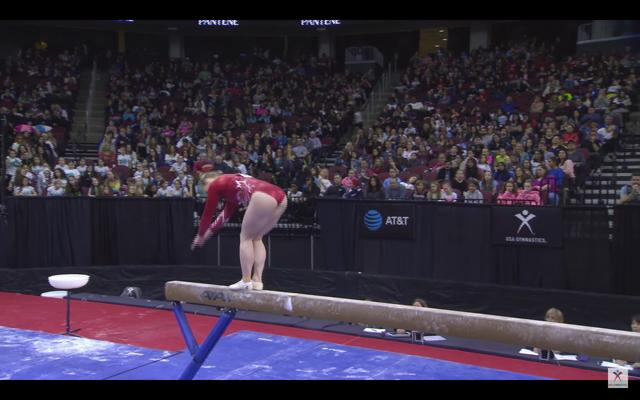
\includegraphics[scale = 0.5]{1} \\
Location of one window from frame 1 to 6: \\
NOTE: The window is only moving slightly from frame to frame because the turtle is only moving a little from frame to frame. \\
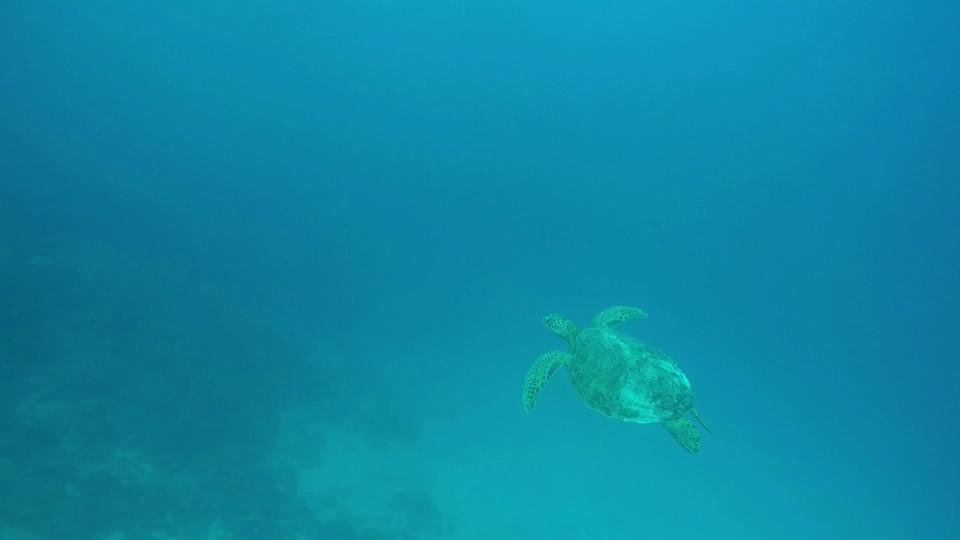
\includegraphics[scale = 0.27]{2} 
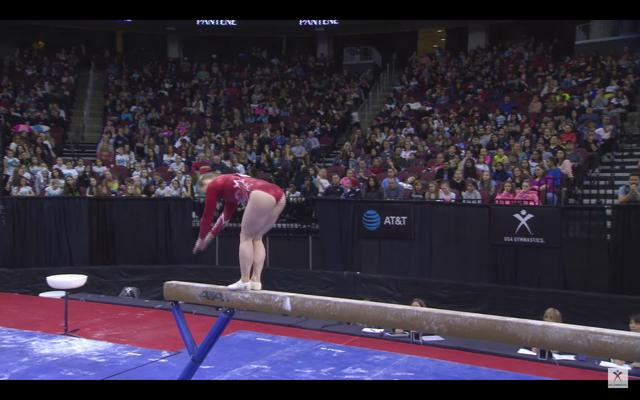
\includegraphics[scale = 0.27]{3} 
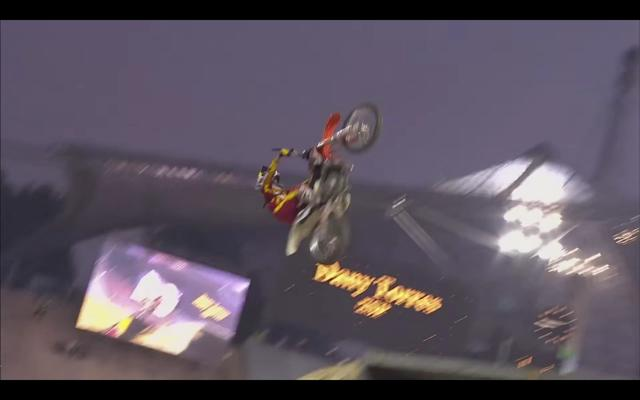
\includegraphics[scale = 0.27]{4} 
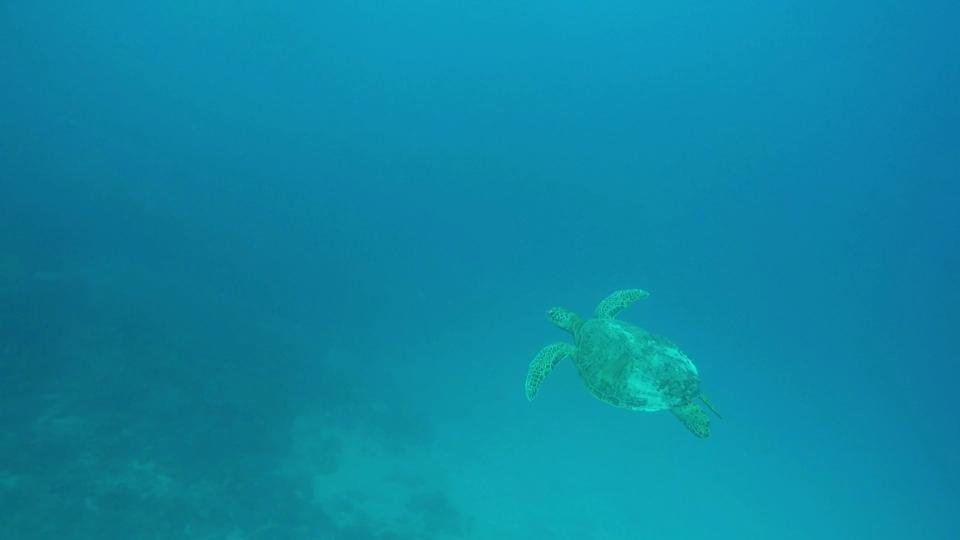
\includegraphics[scale = 0.27]{5} 
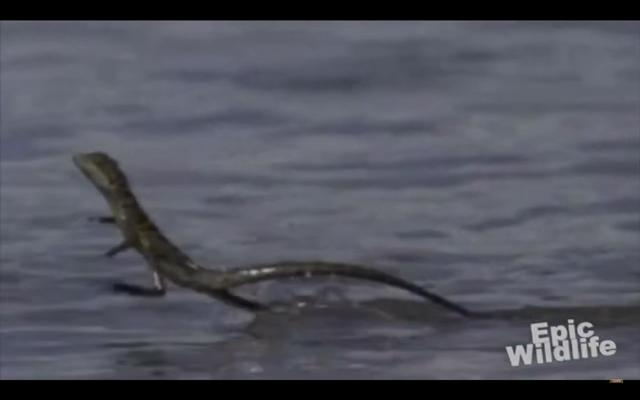
\includegraphics[scale = 0.27]{6}
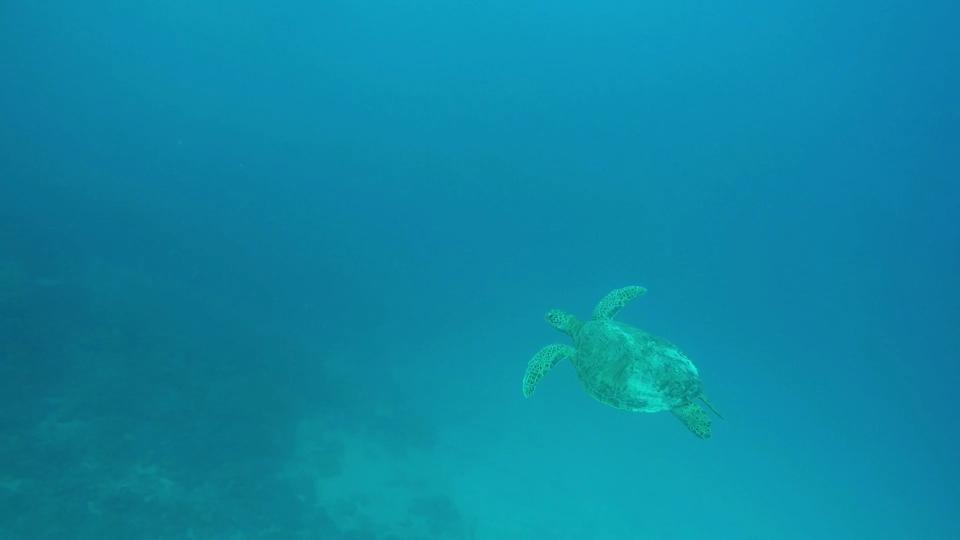
\includegraphics[scale = 0.27]{7} \\
\pagebreak

Color models of one window from frame 1 to 6: \\
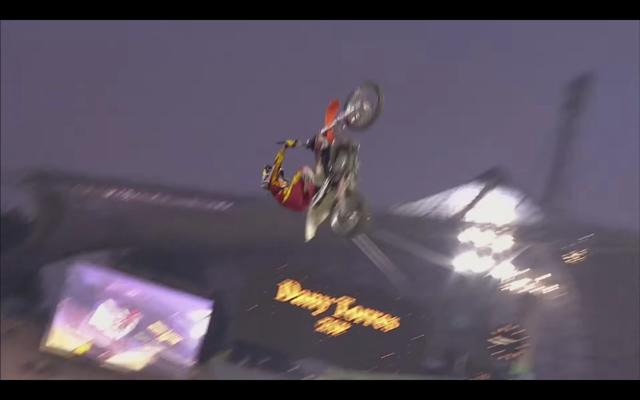
\includegraphics[scale = 0.27]{8} 
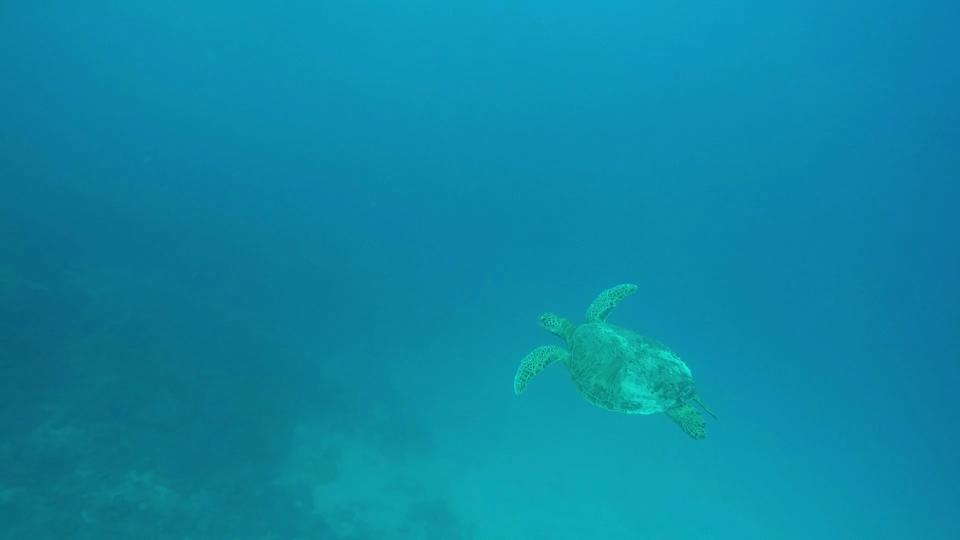
\includegraphics[scale = 0.27]{9} 
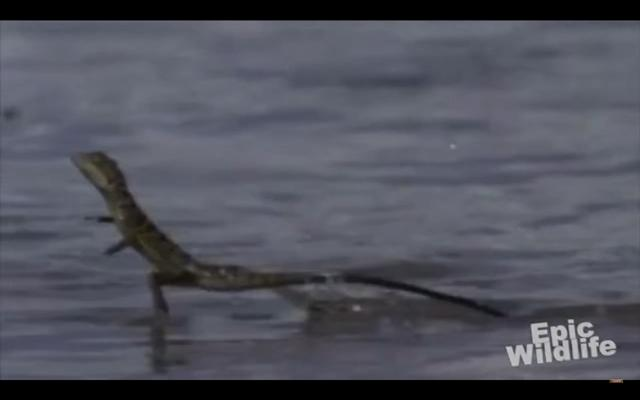
\includegraphics[scale = 0.27]{10} 
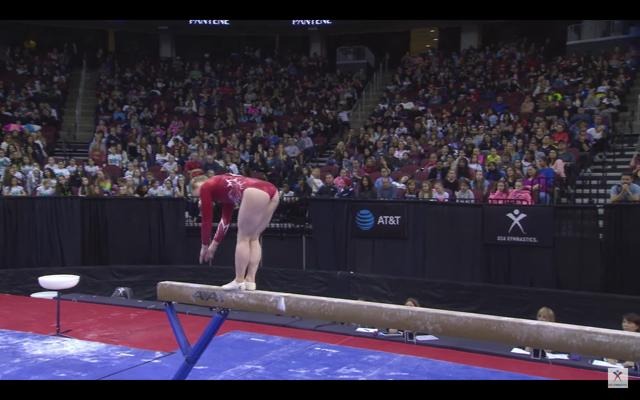
\includegraphics[scale = 0.27]{11} 
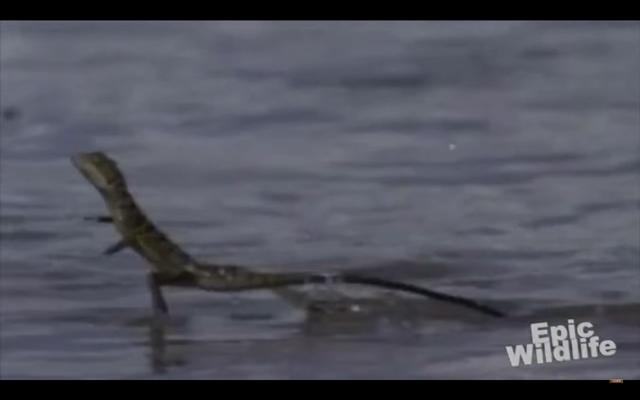
\includegraphics[scale = 0.27]{12}
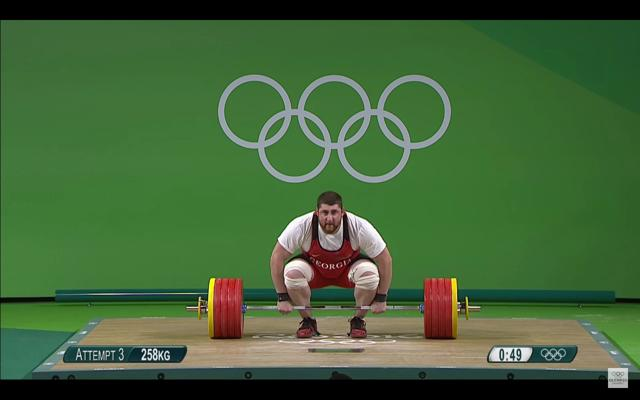
\includegraphics[scale = 0.27]{13} \\
Shape models of one window from frame 1 to 6: \\ 
NOTE: Even though the window is capturing more of the fin in the actual image, it doesn't look like it in the shape model because it is not altered by optical flow, only rigid motion. \\
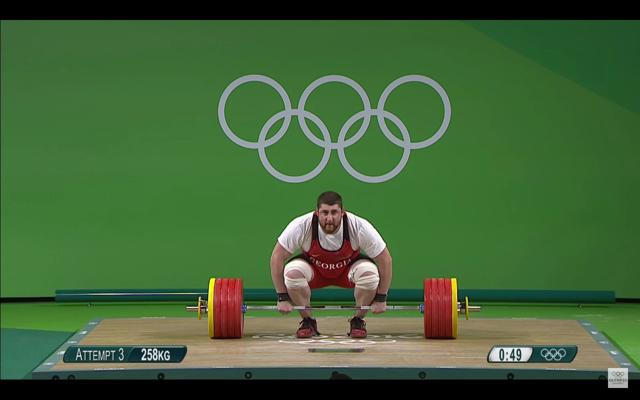
\includegraphics[scale = 0.27]{14} 
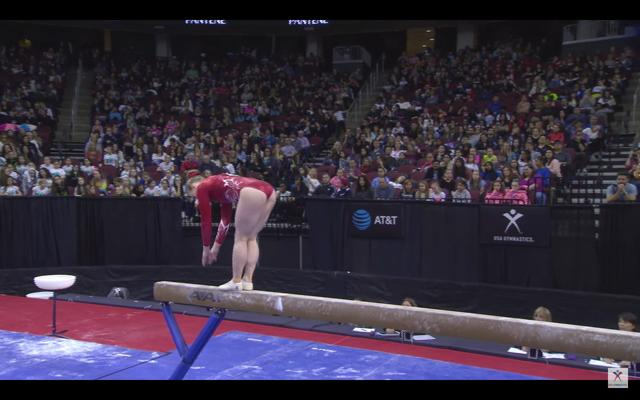
\includegraphics[scale = 0.27]{15} 
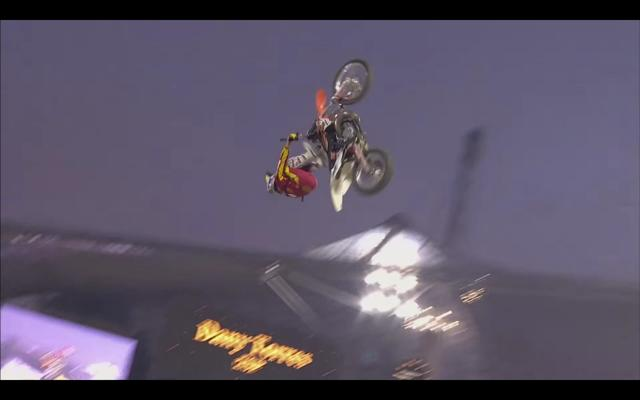
\includegraphics[scale = 0.27]{16} 
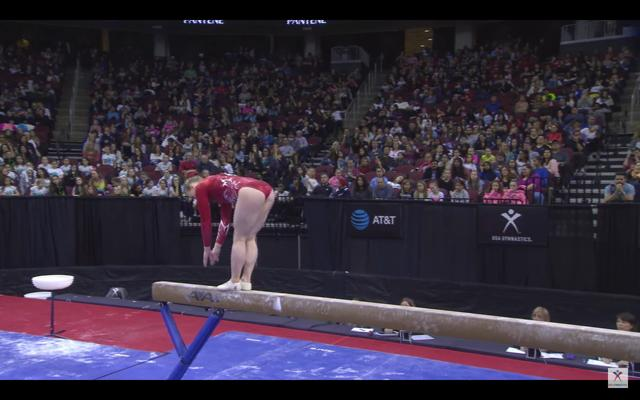
\includegraphics[scale = 0.27]{17} 
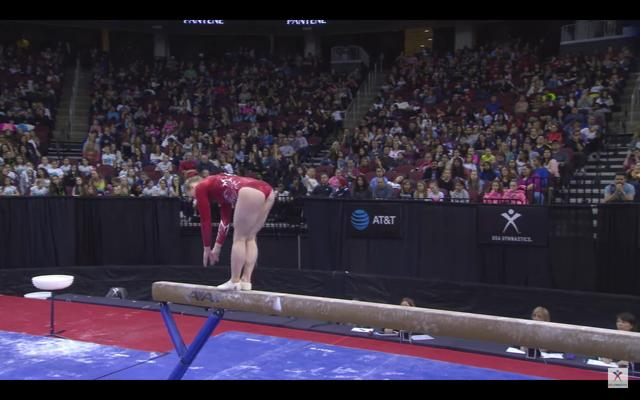
\includegraphics[scale = 0.27]{18}
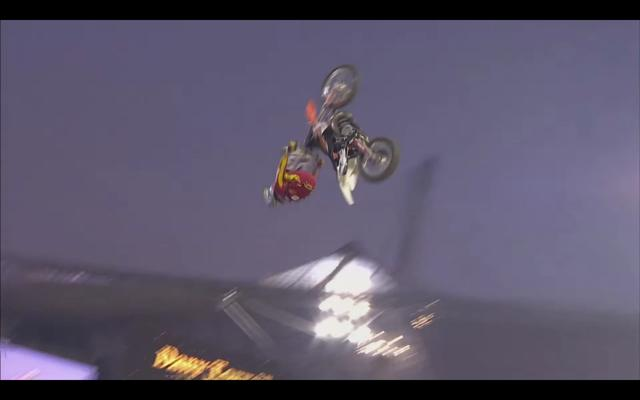
\includegraphics[scale = 0.27]{19} \\
\pagebreak

Shape confidence models of one window from frame 1 to 6: \\ 
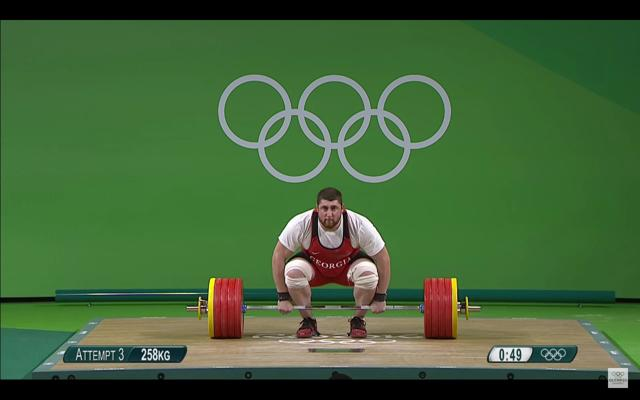
\includegraphics[scale = 0.27]{20} 
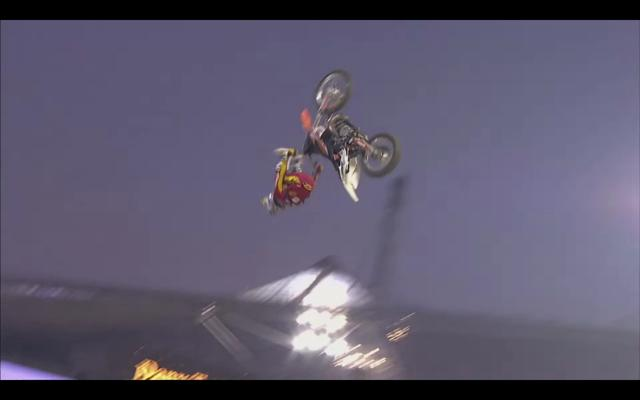
\includegraphics[scale = 0.27]{21} 
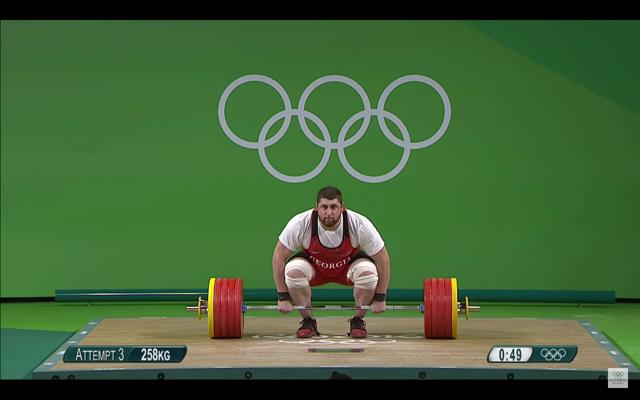
\includegraphics[scale = 0.27]{22} 
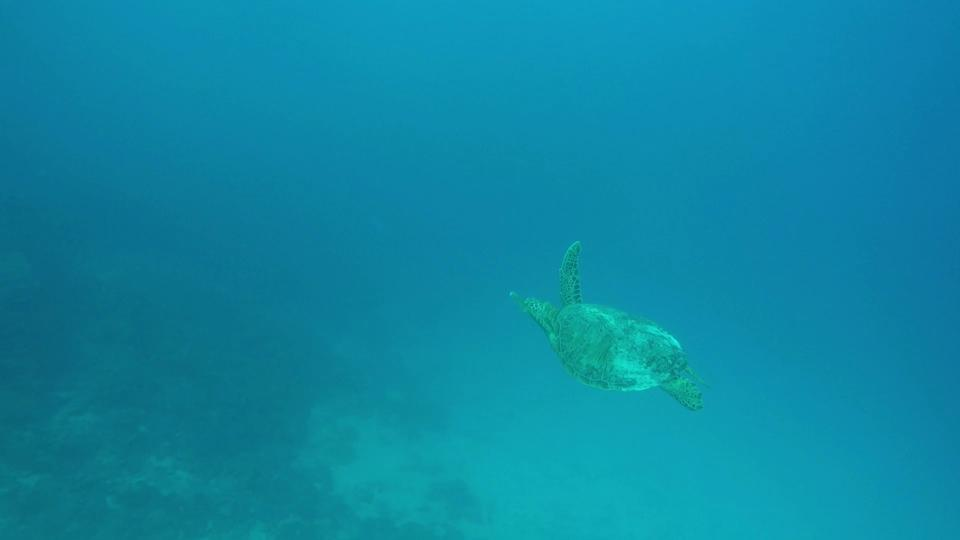
\includegraphics[scale = 0.27]{23} 
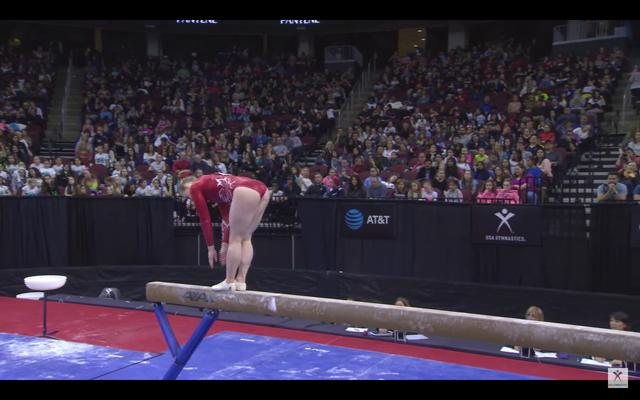
\includegraphics[scale = 0.27]{24}
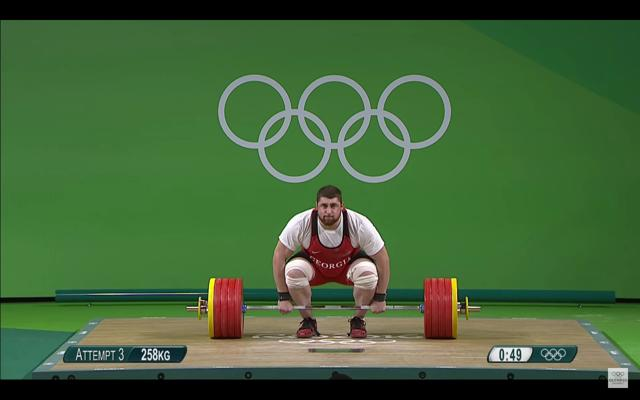
\includegraphics[scale = 0.27]{25} \\
Merged color and shape model of one window from frame 1 to 6: \\
NOTE: There is not one for the first frame because there is not supposed to be one for the first frame. \\
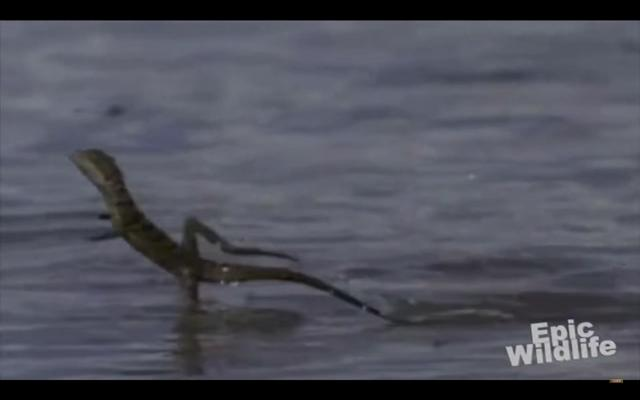
\includegraphics[scale = 0.27]{26} 
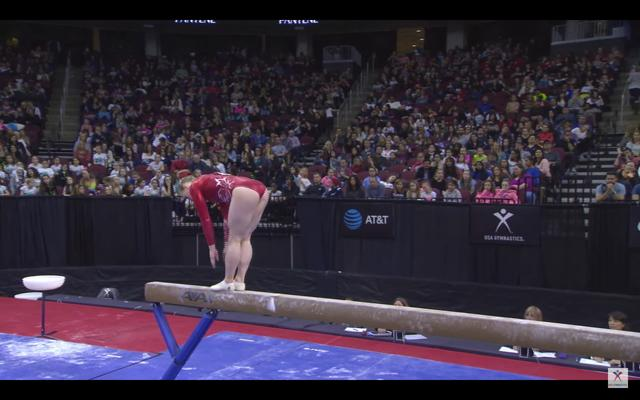
\includegraphics[scale = 0.27]{27} 
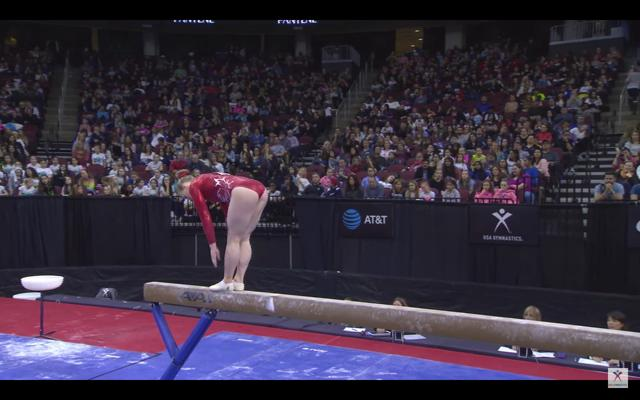
\includegraphics[scale = 0.27]{28} 
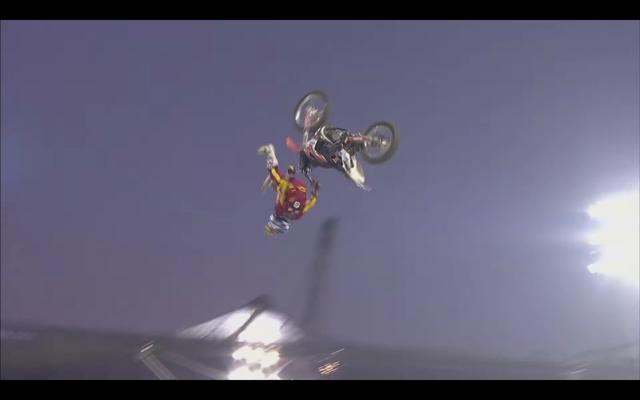
\includegraphics[scale = 0.27]{29}
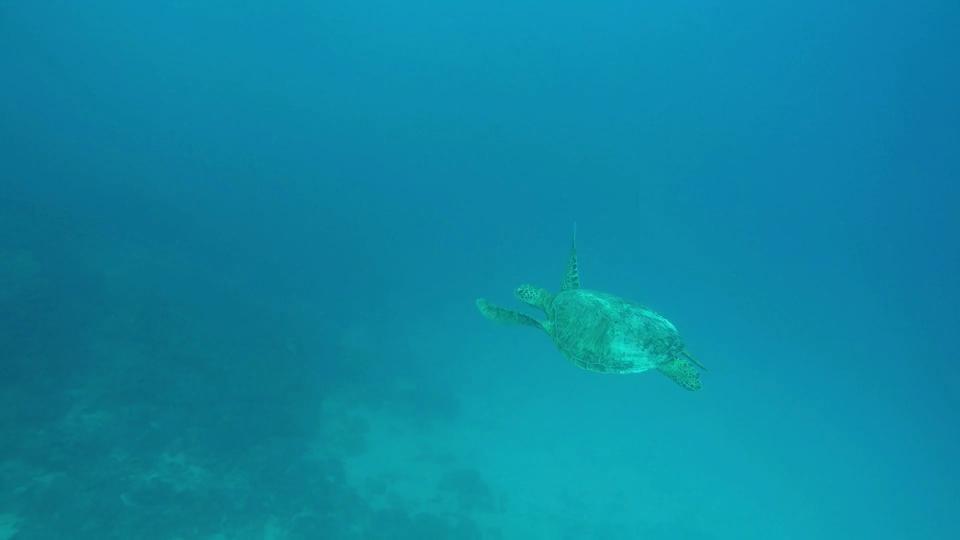
\includegraphics[scale = 0.27]{30} \\
\pagebreak

Final object boundary from frame 1 to 6: \\ 
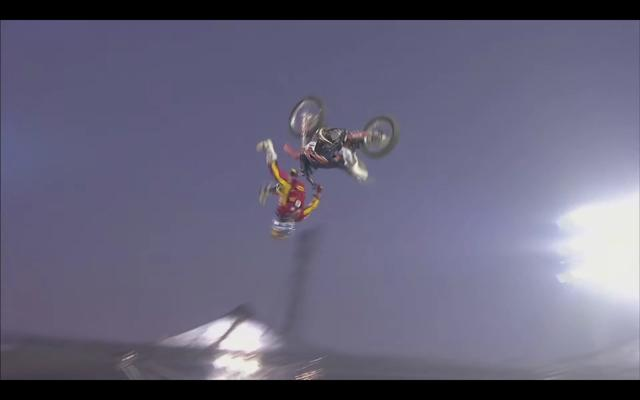
\includegraphics[scale = 0.35]{31} 
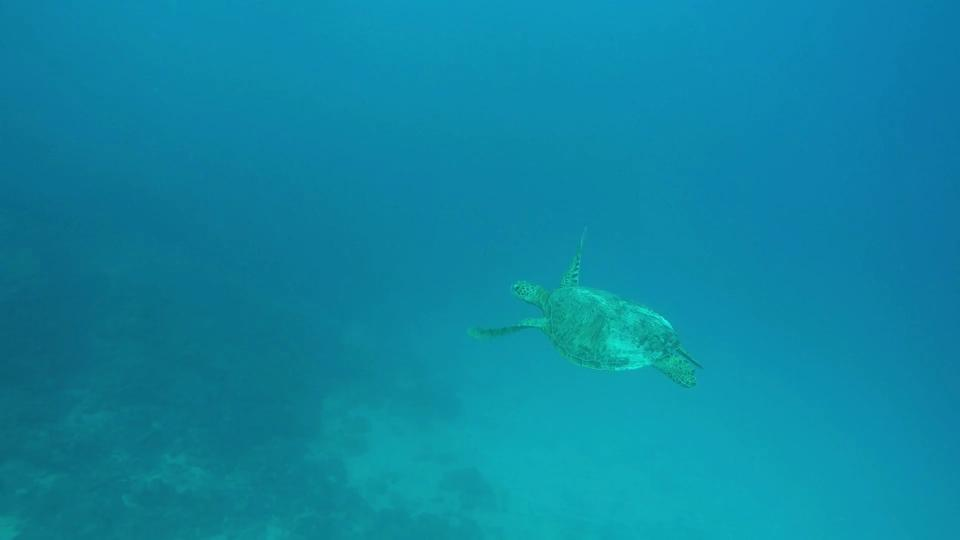
\includegraphics[scale = 0.35]{32} \\
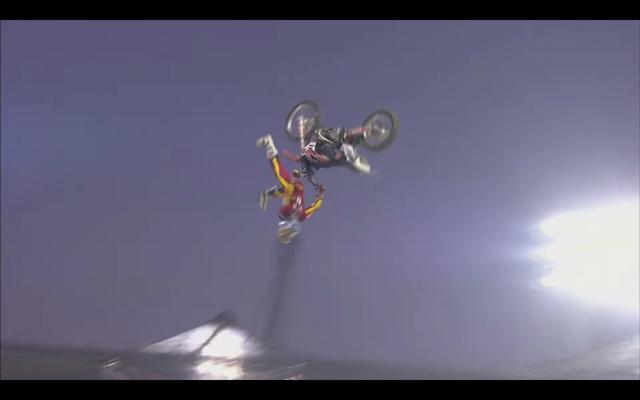
\includegraphics[scale = 0.35]{33} 
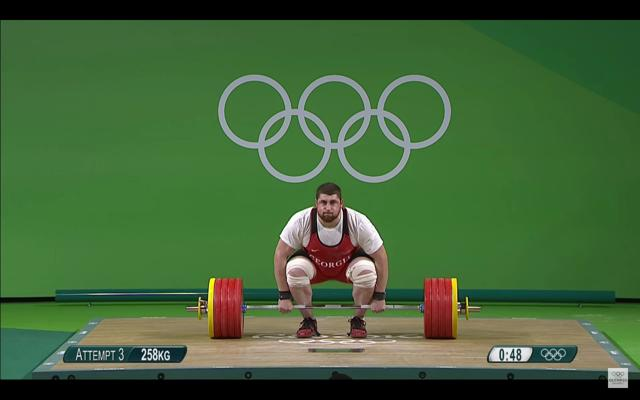
\includegraphics[scale = 0.35]{34} \\
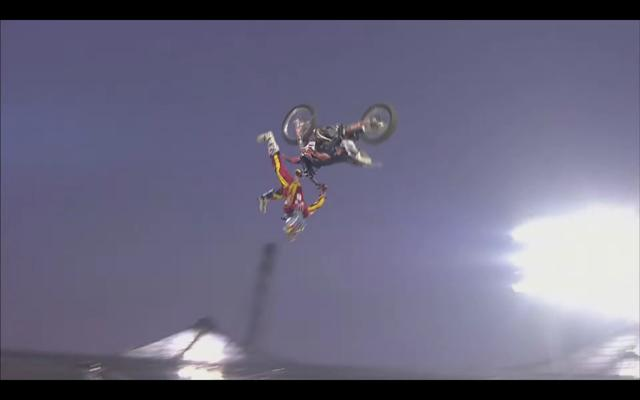
\includegraphics[scale = 0.35]{35}
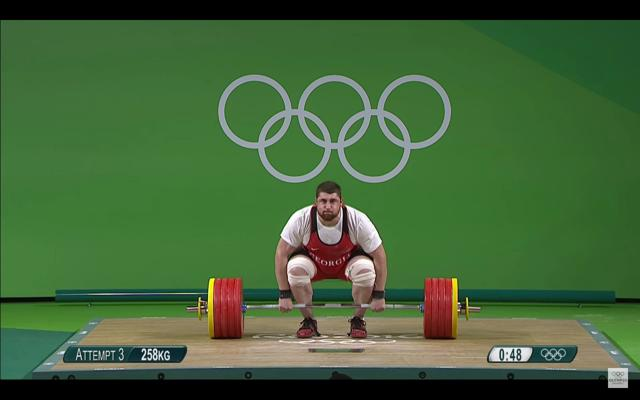
\includegraphics[scale = 0.35]{36} \\
\pagebreak

\subsection{Problems}
There's a few problems that my implementation runs into. First of all, the final outline around the foreground for each frame can be a little off. This is partly due to $lazysnapping$, but my implementation is also to blame. Because the shape model is not shifted by optical flow, only by rigid motion, error builds up and it ends up being more and more off every frame. You can see this above. The window on the sixth frame encompasses all of the end of the right fin. However if you look at the shape model/shape confidence model it looks like it only covers the top half. Since the color model doesn't have a high enough confidence, the shape model is more dominant and results in an incorrect mask when merged. It usually isn't too big of a problem - $lazysnapping$ will get most of the foreground missed - but the problem builds up over frames. This can be seen in the biker video. At first it's fine. It's even good enough when the biker is in the air. However, on the way back down, the outline is focused mainly on the bike and then it shrinks until its nothing. After some digging I found that the windows were not moving as expected and grouped up in a line, which created a smaller final foreground mask than what should have been created. Unfortunately, I could not remedy this issue by the deadline. The following is some pictures from the biker image set:\\
\includegraphics[scale = 0.5]{a1} 
\includegraphics[scale = 0.5]{a2} \\
\includegraphics[scale = 0.5]{a3} 
\includegraphics[scale = 0.5]{a4} \\
I also run into trouble when not enough points can be matched or when optical flow can't be calculated accurately. This seems to happen when the foreground moves position over some frames. In the image set with the gymnast, when she begins her backwards motion, her hands and body become blurry and are unable to be tracked. She also moves from the left to right. Again, this is the same problem as with the biker. Windows are not moving as expected and creating a bad foreground image. In the video (3rd one) you can see that the windows sort of stay in the same place relative to the background, not the foreground. As a result, the program loses where the foreground (the gymnast) is and gives an inaccurate or no outline. \\
%%%%%%%%%%%%%%%%%%%%%%%%%%%%%%%%%%%%%%%%%%%%%%%%%%%%%







\end{document}